\begin{figure}
    \centering
    \caption{Showcase of KL-Divergence of three different normal distributions. The divergence between two normal distributions can occur in both mean and variance. Mean (or expectation) is the center of the distribution, while variance is the spread of the distribution.}
    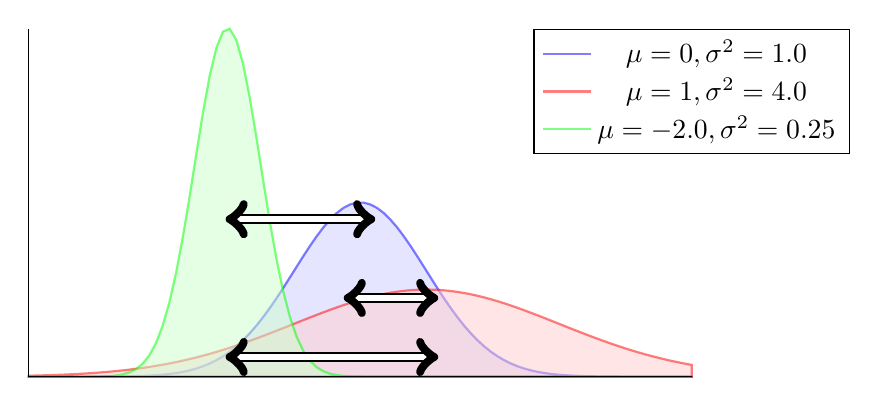
\begin{tikzpicture}
        \begin{axis} [
          no markers, 
          domain=-5:5, 
          samples=100,
          axis lines*=left, 
          height=6cm, 
          width=10cm,
          xtick=\empty, 
          ytick=\empty,
          enlargelimits=false, 
          clip=false, 
          axis on top,
          grid = major,
          legend style={at={(1,1)}, anchor=north, legend columns=1},
        ]

        % Define variables (mean, variance)
        \pgfmathsetmacro{\muA}{0}
        \pgfmathsetmacro{\sigmaA}{1}
        \pgfmathsetmacro{\varA}{\sigmaA^2}
        
        \pgfmathsetmacro{\muB}{1}
        \pgfmathsetmacro{\sigmaB}{2}
        \pgfmathsetmacro{\varB}{\sigmaB^2}
        
        \pgfmathsetmacro{\muC}{-2}
        \pgfmathsetmacro{\sigmaC}{0.5}
        \pgfmathsetmacro{\varC}{\sigmaC^2}
    
        % Blue
        \addplot[blue, thick, fill=blue!20, opacity=0.5] 
        {1/sqrt(2*pi*\sigmaA^2) * exp(-0.5 * ((x-\muA)/\sigmaA)^2)} \closedcycle;
        \addlegendentry{$\mu = \muA, \sigma^2 = \varA$};

        % Red
        \addplot[red, thick, fill=red!20, opacity=0.5] 
        {1/sqrt(2*pi*\sigmaB^2) * exp(-0.5 * ((x-\muB)/\sigmaB)^2)} \closedcycle;
        \addlegendentry{$\mu = \muB, \sigma^2 = \varB$};

        % Green
        \addplot[green, thick, fill=green!20, opacity=0.5] 
        {1/sqrt(2*pi*\sigmaC^2) * exp(-0.5 * ((x-\muC)/\sigmaC)^2)} \closedcycle;
        \addlegendentry{$\mu = \muC, \sigma^2 = \varC$};
        
        \end{axis}

        % Arrows between distributions
        % Blue, Green
        \draw[{<._[sep=-4pt]}-{_[sep=-4pt].>}, line width=0.8pt, double, double distance=2pt] (2.5,2) -- (4.4,2);
        % Green, Red
        \draw[{<._[sep=-4pt]}-{_[sep=-4pt].>}, line width=0.8pt, double, double distance=2pt] (2.5,0.25) -- (5.2,0.25);
        % Blue, Red
        \draw[{<._[sep=-4pt]}-{_[sep=-4pt].>}, line width=0.8pt, double, double distance=2pt] (4,1) -- (5.2,1);

    \end{tikzpicture}
    \label{fig:kl_divergence}
\end{figure}